% !TeX root = ../libro.tex
% !TeX encoding = utf8
\chapter{Relación entre ecuaciones diferenciales y ecuaciones de Volterra}
A continuación veremos la relación que existe entre ambos tipos de ecuaciones, más concretamente, veremos las ecuaciones diferenciales lineales como un caso particular de las ecuaciones de Volterra (lineales) de segunda clase. Primero vamos a ver el caso escalar, y después lo haremos vectorialmente.
\section{Ecuación escalar}
Consideramos el PVI:
\begin{equation}
	x \in \mathcal{C}^1(0,B):\left\lbrace\begin{array}{c} x'(t) = a(t)x(t)+b(t) \\ x(0) = x_0 \end{array}\right.,\qquad t \in (0,B),
\end{equation}
donde $a,b \in \mathcal{C}[0,B]$ y $x_0 \in \R$.
La solución del PVI es el único punto fijo del operador lineal y continuo $T$, definido como
\begin{equation}
	T: \mathcal{C}[0,B] \longrightarrow \mathcal{C}[0,B]
\end{equation}
\begin{equation}
	\qquad \qquad x \longmapsto T(x): [0,B] \rightarrow \R
\end{equation}
\begin{equation}
	\qquad \qquad \qquad \qquad \qquad \qquad \qquad \qquad (T(x))(t) = x_0 + \int_0^t(a(s)x(s)+b(s))ds.
\end{equation}
Por tanto, vemos que la solución del PVI es un caso particular de la ecuación integral lineal de Volterra de segunda clase:
\begin{equation}
	x(t) = f(t) + \int_0^t K(t,s)x(s)ds,
\end{equation}
donde
\begin{equation}
	f(t) = x_0 + \int_0^t b(s)ds, \qquad K(t,s) = a(s).
\end{equation}
Para ver la equivalencia, basta aplicar el Teorema Fundamental del Cálculo a la siguiente ecuación integral:
\begin{equation}
	x(t) = x_0 + \int_0^t (a(s)x(s)+b(s))ds,
\end{equation}
donde $x \in \mathcal{C}[0,B]$, y obtenemos, equivalentemente,
\begin{equation}
	\left\lbrace\begin{array}{c} x'(t) = a(t)x(t)+b(t) \\ x(0) = x_0 \end{array}\right.,\qquad t \in (0,B),
\end{equation}
siendo $x \in \mathcal{C}^1[0,B]$. En definitiva, la solución del PVI inicial coincide con la solución de la ecuación de Volterra lineal de segunda clase.
\section{Ecuación vectorial}
En este caso, el PVI sería:
\begin{equation}\label{eq:vect}
 \hspace*{-3cm} 	\begin{array}{c} \textbf{x} \in \mathcal{C}^1([0,B],\R^n) \\ \textbf{x}:[0,B] \longrightarrow \R^n \\ \qquad \qquad \qquad \qquad t \longmapsto \textbf{x}(t) = (x_1(t),...,x_n(t)) \end{array}:\left\lbrace\begin{array}{c} x_1'(t) = a_{11}(t)x_1(t)+\cdots+a_{1n}(t)x_n(t)+b_1(t) \\ \vdots \\ x_n'(t) = a_{n1}(t)x_1(t)+\cdots+a_{nn}(t)x_n(t)+b_n(t) \\ x_1(0) = x_1,...,x_n(0) =x_n, \end{array}\right.
\end{equation}
donde $a_{ij} \in \mathcal{C}([0,B])$ y $b_i \in \mathcal{C}([0,B])$ para todo $i,j \in \{1,...,n\}$. Utilizando notación matricial para simplificar las fórmulas, nos quedaría de la siguiente forma:
\begin{equation}
	\begin{array}{c}
		\textbf{x}'(t) = \textbf{A}(t)\textbf{x}(t)+\textbf{b}(t) \\ \textbf{x}(0) = \textbf{x}_\textbf{0}
	\end{array}
\end{equation}
donde
\begin{equation}
	\textbf{A}(t) = \begin{pmatrix}
		a_{11}(t) & \cdots & a_{1n}(t)\\ 
		\vdots & & \vdots \\
		a_{n1}(t) & \cdots & a_{nn}(t)
	\end{pmatrix}, \qquad \textbf{x}(t) = \begin{pmatrix}
	x_1(t) \\ \vdots \\ x_n(t)
	\end{pmatrix}, \qquad \textbf{b}(t) = \begin{pmatrix}
	b_1(t) \\ \vdots \\ b_n(t)
	\end{pmatrix}
\end{equation}
y el vector $\textbf{x}_\textbf{0}$ está formado por los valores iniciales de cada una de las ecuaciones.

La solución de este PVI viene dada por el punto fijo del operador lineal y continuo
\begin{equation}
	\begin{array}{c}
		\textbf{T}: (\mathcal{C}[0,B], \R^n) \longrightarrow \mathcal{C}([0,B],\R^n) \\  \textbf{x} \longmapsto \textbf{Tx}:[0,B] \longrightarrow \R^n \\  \qquad \qquad \qquad \qquad \qquad \textbf{Tx}(t)= \textbf{x}_\textbf{0} + \int_0^t (\textbf{A}(s)\textbf{x}(s)+\textbf{b}(s))ds.
	\end{array}
\end{equation}
Luego al igual que en el caso escalar, la solución del PVI es un caso particular de la ecuación de Volterra de segunda clase
\begin{equation}
	\textbf{x}(t) = \textbf{f}(t) + \int_0^t \textbf{K}(t,s)\textbf{x}(s)ds.
\end{equation}
Ahora vemos la equivalencia aplicando el Teorema Fundamental del Cálculo a cada uno de los elementos de la matriz y de los vectores de la siguiente ecuación:
\begin{equation}
	\textbf{x}(t)= \textbf{x}_\textbf{0} + \int_0^t (\textbf{A}(s)\textbf{x}(s)+\textbf{b}(s))ds,
\end{equation}
obteniendo:
\begin{equation}
	\begin{array}{c}
		\textbf{x}'(t) = \textbf{A}(t)\textbf{x}(t)+\textbf{b}(t) \\ \textbf{x}(0) = \textbf{x}_\textbf{0}.
	\end{array}
\end{equation}
Es decir, tanto de forma escalar como vectorial, tenemos el siguiente resultado.
\begin{corolario}
	La solución del PVI~\eqref{eq:vect} coincide con la solución de la ecuación integral lineal de Volterra de segunda clase dada por
	\begin{equation}
		\textbf{x}(t)= \textbf{x}_\textbf{0} + \int_0^t (\textbf{A}(s)\textbf{x}(s)+\textbf{b}(s))ds.
	\end{equation}
\end{corolario}

Vamos a ver un ejemplo en el cual, partiendo de un PVI formado por un sistema de ecuaciones, lo transformaremos en un sistema de ecuaciones integrales de Volterra, y posteriormente, lo resolveremos mediante el método de aproximaciones sucesivas, luego lo volveremos a resolver utilizando el programa \textit{Maxima}, y por último, compararemos los resultados obtenidos.

\begin{ejemplo}
	Consideramos el PVI
	\begin{equation}
		\begin{dcases} x'(t) = \dfrac{x(t)}{7}-\dfrac{y(t)}{10} + t \\ y'(t) = -\dfrac{x(t)}{8} +\dfrac{y(t)}{9} +1 \\ x(0) = 0, \qquad y(0) = 0 \end{dcases}, \qquad t \in [0,1],
	\end{equation}
	que, como hemos visto anteriormente, es equivalente a la siguiente ecuación de Volterra:
	\begin{equation}
		\textbf{x}(t)= \textbf{x}_\textbf{0} + \int_0^t (\textbf{A}(s)\textbf{x}(s)+\textbf{b}(s))ds.
	\end{equation}
	donde
	\begin{equation}
		\textbf{A}(t) = \begin{pmatrix}[1.5]
			1/7 & -1/10 \\ 
			-1/8 & 1/9
		\end{pmatrix}, \qquad \textbf{x}(t) = \begin{pmatrix}
			x(t) \\ y(t)
		\end{pmatrix}, \qquad \textbf{b}(t) = \begin{pmatrix}
			t \\ 1
		\end{pmatrix}, \qquad \textbf{x}_\textbf{0} = \begin{pmatrix}
		0 \\ 0
		\end{pmatrix}.
	\end{equation}
	Así, aplicaremos la siguiente fórmula iterativa para calcular las aproximaciones sucesivas:
	\begin{equation}
		\textbf{x}_{n+1}(t) = \textbf{f}(t) + \int_0^t \textbf{K}(s,t)\textbf{x}_n(s)ds, \qquad n \geqslant 0.
	\end{equation}
	donde
	\begin{equation}
		\textbf{f}(t) = \textbf{x}_\textbf{0} + \int_0^t \textbf{b}(s)ds, \qquad \textbf{K}(t,s) = \textbf{A}(s),
	\end{equation}
	sustituimos $\textbf{x}_\textbf{0}$ y obtenemos:
	\begin{equation}
		\textbf{x}_{1}(t) = \textbf{f}(t) + \int_0^t \textbf{K}(s,t)\textbf{x}_0(s)ds = \begin{pmatrix}[1.7]	\dfrac{t^2}{2} \\ t 	\end{pmatrix},
	\end{equation}
	en la segunda iteración tenemos
	\begin{equation}
		\textbf{x}_{2}(t) = \textbf{f}(t) + \int_0^t \textbf{K}(s,t)\textbf{x}_1(s)ds = \begin{pmatrix}[2.2] \dfrac{t^3}{14}+\dfrac{2t^2}{5}\\ -\dfrac{t^3}{16}+\dfrac{t^2}{9}+t	\end{pmatrix},
	\end{equation}
	Así, llegamos a que la iteración número cinco es:
	\begin{equation}
		\textbf{x}_5(t) = \begin{pmatrix}[2.2]
			\dfrac{2351441t^6}{2489356800}+\dfrac{494317t^5}{200037600}+\dfrac{8209t^4}{793800}+\dfrac{29t^3}{630}+\dfrac{2t^2}{5}   \\ -\dfrac{9169t^6}{10001880}-\dfrac{1232909t^5}{514382400}-\dfrac{4057t^4}{408240}-\dfrac{61t^3}{1620}+\dfrac{t^2}{9}+t
		\end{pmatrix}
	\end{equation}
	Ahora vamos a obtener la solución exacta gracias a Maxima, mediante los comandos que vemos en la \autoref{fig:maxima1}
	\begin{figure}[h!]
		\centering
		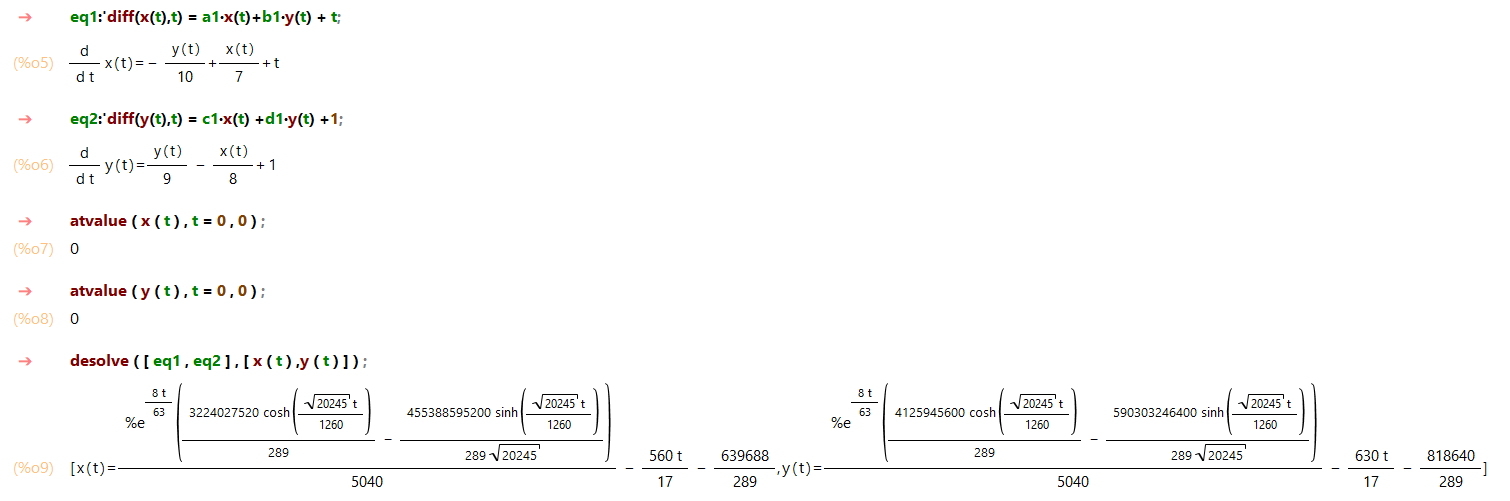
\includegraphics[width=\textwidth]{maxima1}
		\caption{Comandos de Maxima para obtener la solución exacta}
		\label{fig:maxima1}
	\end{figure}
	, finalmente comparamos los resultados para $x(t)$ (\autoref{fig:solx}), en azul vemos la solución del método de las aproximaciones sucesivas, y en rojo la solución de Maxima, de la misma forma para $y(t)$ (\autoref{fig:soly}).
	\begin{figure}[h!]
		\centering
		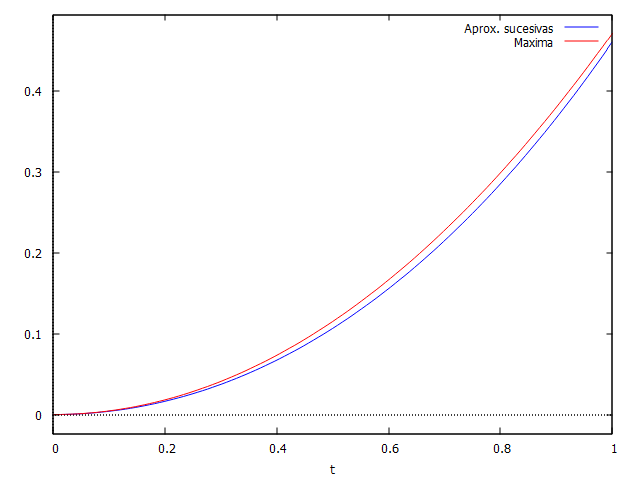
\includegraphics[width=0.8\textwidth]{compx}
		\caption{Solución $x(t)$}
		\label{fig:solx}
	\end{figure}
	\begin{figure}[h!]
		\centering
		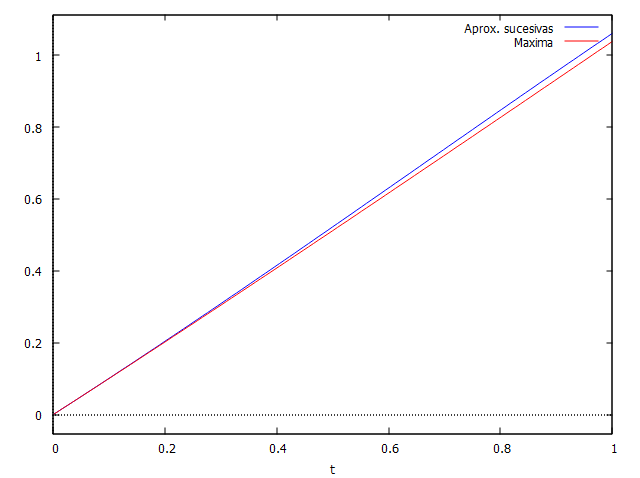
\includegraphics[width=0.8\textwidth]{compy}
		\caption{Solución $y(t)$}
		\label{fig:soly}
	\end{figure}
	Vemos claramente cómo con $5$ iteraciones, la convergencia es bastante buena y obtenemos una solución muy cercana a la exacta.
\end{ejemplo}
\endinput
%------------------------------------------------------------------------------------
% FIN DEL CAPÍTULO. 
%----------------------------------------------------------------------------------
-